\documentclass[11pt]{article}

\usepackage{fullpage}
\usepackage[round,semicolon]{natbib}
\usepackage{amssymb}
\usepackage{amsmath}
\usepackage{bbm}
\usepackage{graphicx}
\usepackage{hyperref}

\DeclareMathOperator{\erf}{erf}
\DeclareMathOperator{\lngamma}{\ln\!\Gamma}

% NOTE
% one sentence per line for nice git diffs
% WD: I'm a fan of initialed source comments like this

\title{Coalescent inference of mutation spectrum histories from sample frequency spectra}

\author{
W. DeWitt$^{1}$, K. Harris$^{2}$, and K. Harris$^{1}$\\
\small{Departments of $^1$Genome Sciences and $^2$Biology, University of Washington, Seattle, USA}
% \small{$^\ast$ Equal contribution}
}

\begin{document}

\maketitle

\begin{abstract}

Single nucleotide variant (SNV) frequencies partitioned according to triplet nucleotide context vary among human ancestry groups and among great ape species, indicating variation and divergence of the mutation process.
The sample frequency spectrum (SFS)---the distribution of derived allele frequencies among sampled haplotypes---is a well-studied population genetic summary statistic that is sensitive to demographic history.
We extend a coalescent framework for demographic inference from the SFS to accommodate inference of mutation spectrum histories from the triplet-resolved sample frequency spectrum (3-SFS).
We formulate inference of mutation spectrum histories from the 3-SFS as a linear inverse problem.

\end{abstract}


\section{Introduction}\label{sec:intro}

\cite{Harris2017-fw} showed triplet SNV spectrum differences between human groups and between great apes, and used a coalescent simulation approach to fit the timing of a pulse of \texttt{T\underline{C}C>T\underline{T}C} mutations in Europeans.
We develop coalescent theory for the dependence of the expected 3-SFS on both demographic history (effective population size as a function of time into the past) \emph{and} triplet mutation spectrum history (triplet-specific mutation rates as a function of time into the past).
This is similar in spirit to Kelley's simulation-based approach (which assumed the European demography of \cite{Tennessen2012-dq}), but is much faster, more flexibly parameterized, and extendable to joint inference of demographic and mutation spectrum histories.

The setting for our modeling is Kingman's coalescent \citep{Kingman1982-ge, Kingman1982-tf, Kingman1982-ys, Kingman2000-jr}, with all the usual niceties: neutrality, infinite sites, linkage equilibrium, and panmixia.
We will retrace the derivation by \cite{Griffiths1998-qf} of the frequency distribution of a derived allele conditioned on the demographic history, while generalizing to a time inhomogeneous mutation process.
We will make use of important results of \cite{Polanski2003-kg} and \cite{Polanski2003-ll} which facilitate numerical computation under this model, and formulate the expected 3-SFS under piecewise constant demographic and mutation spectrum histories building on the notation of \cite{Rosen2018-bb} for the expected SFS with a piecewise constant demographic history and constant mutation process.


\section{Model}\label{sec:model}

\subsection{The expected SFS given demographic and mutation rate histories}\label{sec:model:xi}

Suppose $n$ haplotypes are sampled in the present, and let rvs $T = T_2,\dots,T_n$ denote the coalescent times measured retrospectively from the present (i.e. $T_n$ is the most recent coalescent time, and $T_2$ is the TMRCA of the sample).
As in \cite{Griffiths1998-qf} \S3, we consider a marked Poisson process in which every mutation is assigned a random label drawn iid from the uniform distribution on $(0,1)$.
This is tantamount to an (uncountably) infinite sites assumption, with the unit interval representing the genome, and the random variate labels representing mutant sites.
Further suppose that mutation rate is not constant, but a specified function of time $\mu(t) \ge 0$ (measured in mutations per genome per generation) applying equally to all lines in the coalescent tree at a given time $t$ (measured retrospectively from the present in units of Wright-Fisher generations).
A given line in the coalescent tree then acquires mutations on a genomic subinterval $(x,x+\delta x)$ at rate $\mu(t)\delta x$.
The following argument can be generalized to a nonuniform distribution of mutation intensity over the genome without changing the results.

\begin{figure}
\centering
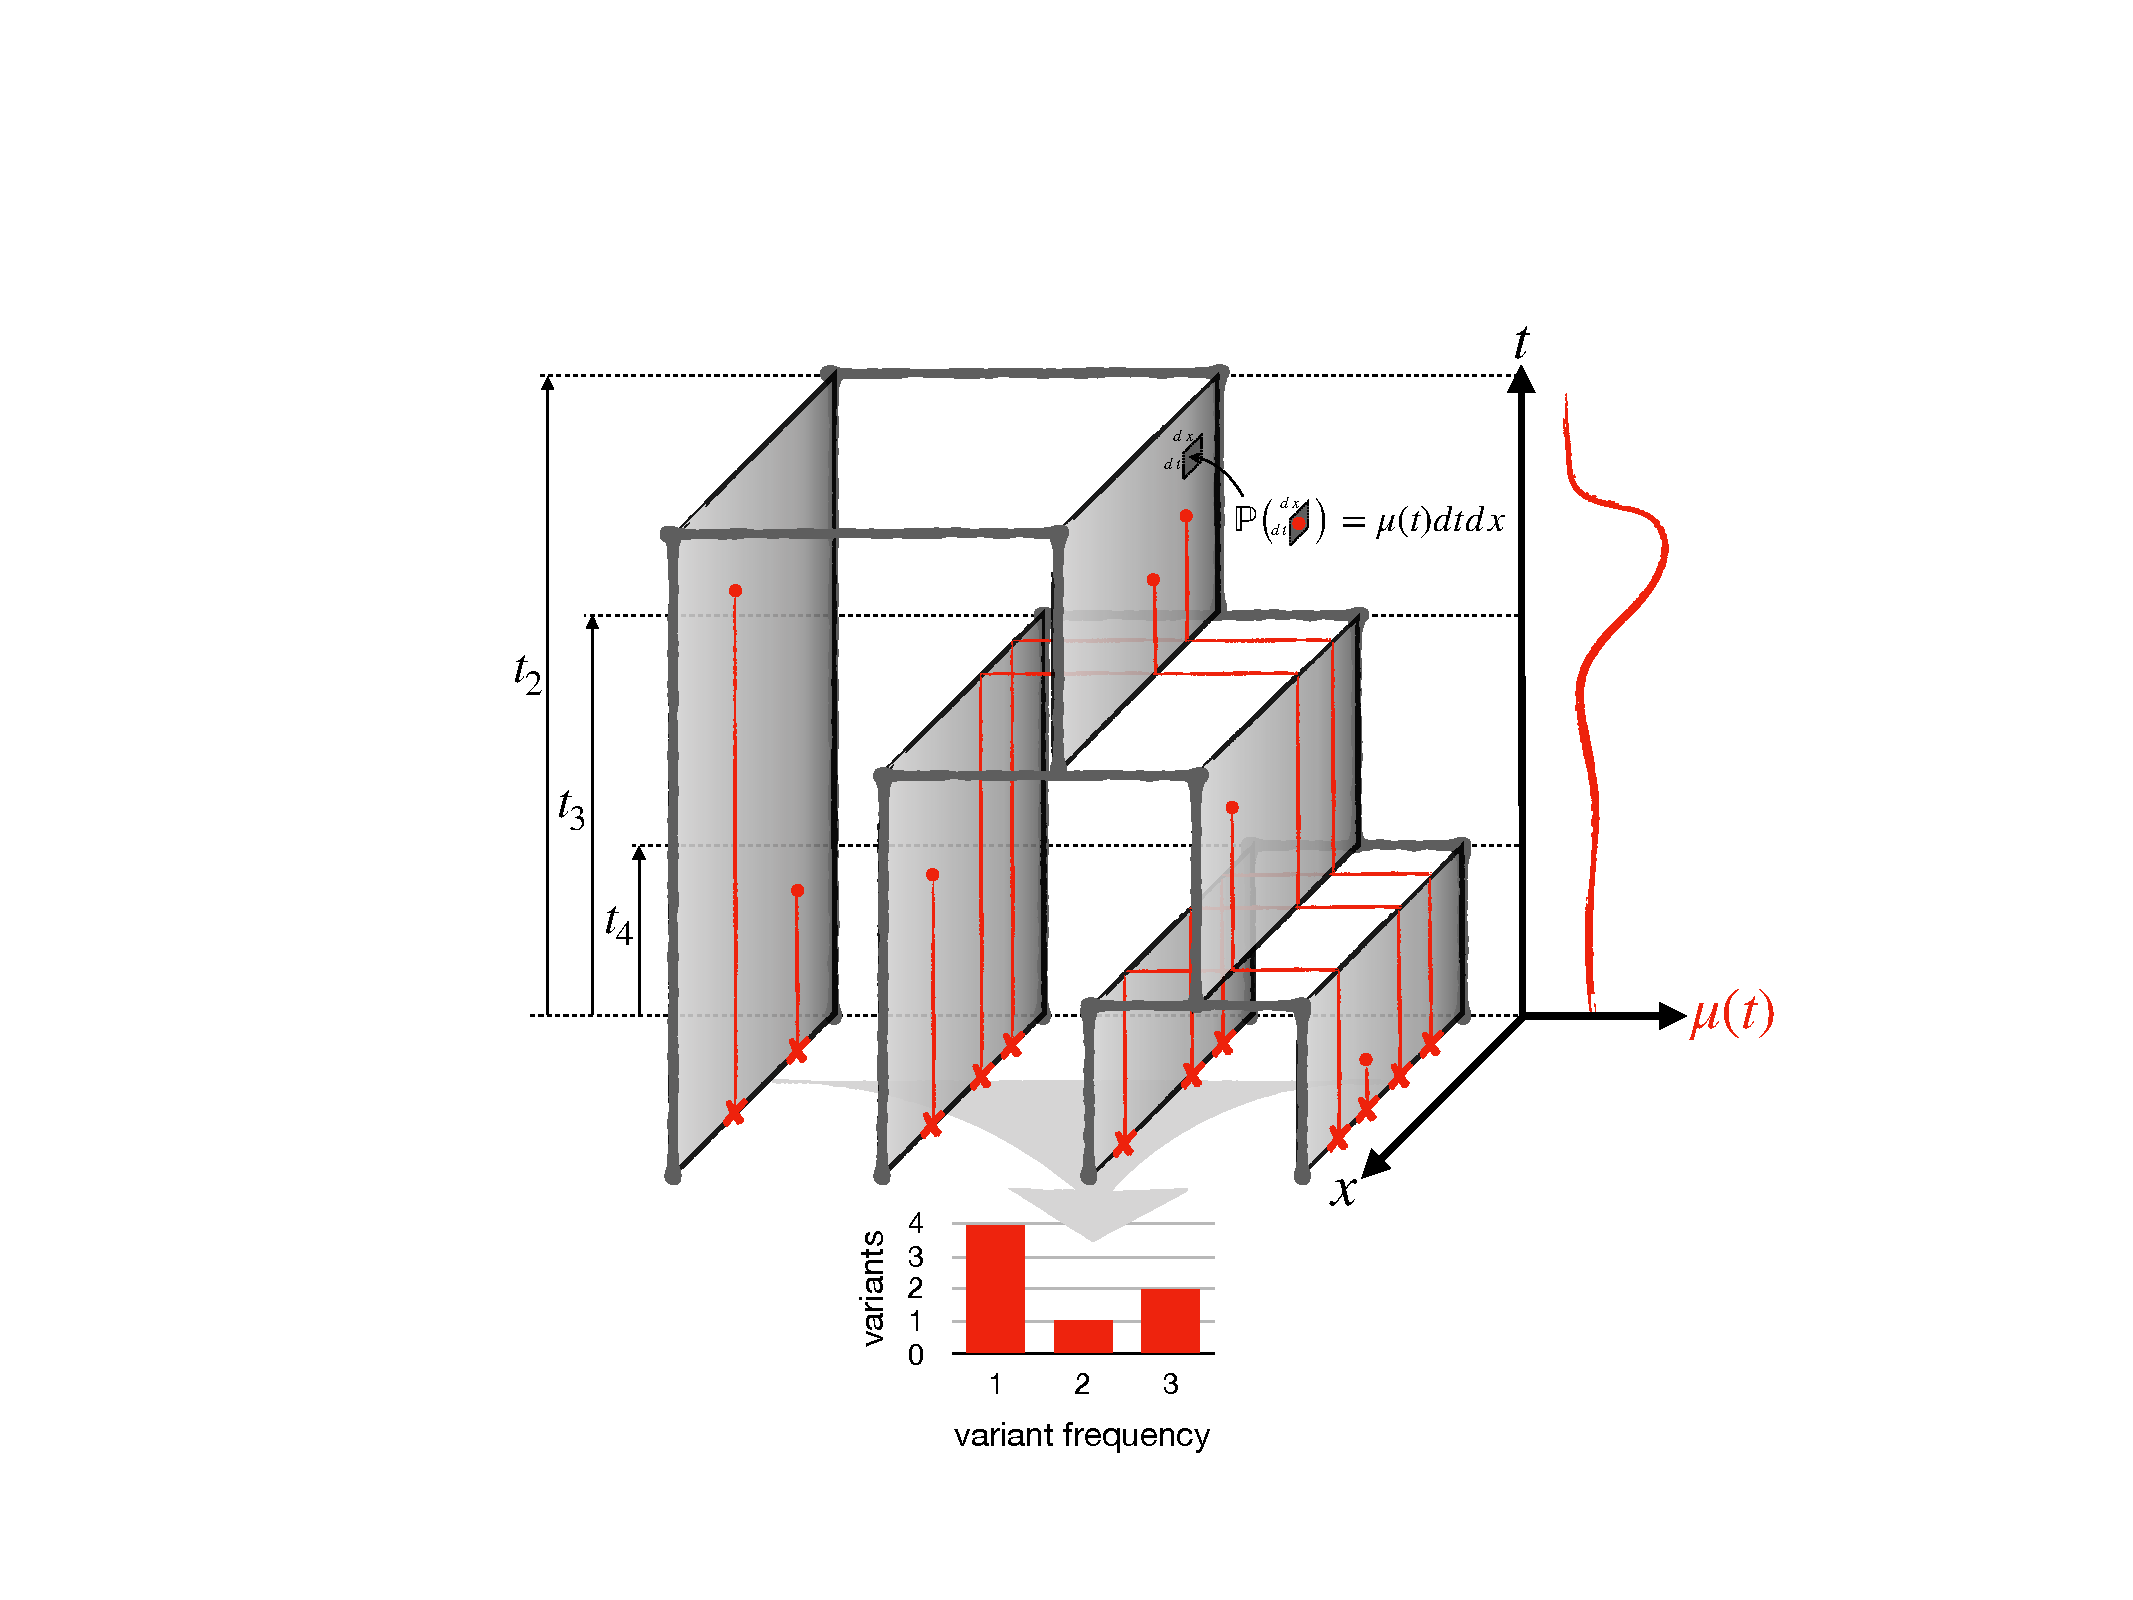
\includegraphics[width=\textwidth]{figures/model}
\caption{Schematic of the marked Poisson process model with $n=4$.
We condition on coalescent times $T_4=t_4,T_3=t_3,T_2=t_2$ and consider mutation intensity function $\mu(t)$.
Red dots indicate mutation events placed by time $t$, genomic position $x$, and coalescent line (which are depicted as extruded in the genomic coordinate axis, grey sheets).
The probability that a differential element $dxdt$ on a given sheet contains a mutation is proportional to the instantaneous mutation intensity $\mu(t)$.
}
\label{fig:model}
\end{figure}

Let rv $\mathcal{E}_{\delta x, b}$ denote the event that a mutation subtending $b$ haplotypes in the sample occurred within a given genomic interval $(x,x+\delta x)$ (identical for all $x$, given the uniform labeling distribution).
Let $I_k$ denote the $k$th intercoalescent time interval, i.e.\ $I_n = (0, T_n),\ I_{n-1} = (T_n, T_{n-1}),\ \dots,\ I_2 = (T_3, T_2)$.
Let rv $\mathcal{E}_{\delta x, b, k}$ denote the event that the mutation $\mathcal{E}_{\delta x, b}$ occurred during $I_k$.
For small $\delta x$ and finite $\mu(t)$ we have
\begin{align*}
\mathbbm{P}(\mathcal{E}_{\delta x, b}\mid T) &= \sum_{k=2}^n \mathbbm{P}(\mathcal{E}_{\delta x, b, k}\mid T)\\
&= \sum_{k=2}^n p_{n,k}(b)\left(k\delta x\int_{t\in I_k}\mu(t)dt + O(\delta x)\right),
\end{align*}
where
\begin{equation}
\label{eqn:p}
p_{n,k}(b) = \frac{\binom{n-b-1}{k-2}}{\binom{n-1}{k-1}}
\end{equation}
is the probability that a mutant that arose when there were $k$ ancestral lines of $n$ sampled haplotypes will be present in $b$ of them (see \cite{Griffiths1998-qf} eqn 1.9), and the quantity in parenthesis is the probability that a mutation arose during the $k$th intercoalescent interval in a small genomic interval of size $\delta x$.
Marginalizing $T$ gives
\begin{align*}
\mathbbm{P}(\mathcal{E}_{\delta x, b}) &\simeq \delta x\sum_{k=2}^n k p_{n,k}(b) \mathbbm{E}_T\left[\int_{t\in I_k}\mu(t)dt\right].
\end{align*}
For small $\delta x$, each such interval contains zero or one mutations, so the expected number of mutations subtending $b$ haplotypes (i.e.\ the $b$th component of the SFS) is
\[
\xi_b = \int d\mathbbm{P}(\mathcal{E}_{dx, b}) = \sum_{k=2}^n k p_{n,k}(b)\mathbbm{E}_T\left[\int_{t\in I_k}\mu(t)dt\right]\nonumber
\]
Using the explicit bounds of the intercoalescent intervals gives
\begin{align}
\label{eqn:xi}
\xi_b &= \sum_{k=2}^n k p_{n,k}(b) \mathbbm{E}_{T_k}\left[\int_0^{T_k}\mu(t)dt\right] - \sum_{k=2}^{n-1} k p_{n,k}(b) \mathbbm{E}_{T_{k+1}}\left[\int_0^{T_{k+1}}\mu(t)dt\right]\nonumber\\
&= \sum_{k=2}^n k p_{n,k}(b) \mathbbm{E}_{T_k}\left[\int_0^{T_k}\mu(t)dt\right] - \sum_{k=3}^{n} (k-1) p_{n,k-1}(b) \mathbbm{E}_{T_{k}}\left[\int_0^{T_k}\mu(t)dt\right]\nonumber\\
&= \sum_{k=2}^n B_{b,k} \mathbbm{E}_{T_k}\left[\int_0^{T_k}\mu(t)dt\right],
\end{align}
where
\begin{equation}
\label{eqn:B}
B_{b,k}\equiv
\begin{cases}
k p_{n,k}(b),& k=2\\
k p_{n,k}(b) - (k-1) p_{n,k-1}(b),& k > 2
\end{cases}
\end{equation}

\cite{Polanski2003-kg} (eqns 5-8) give the marginal density for the coalescent time $T_k$ as
\begin{equation}
\label{eqn:pi}
\pi_k(t_k) = \sum_{j=k}^n A_{k,j} q_j(t_k)
\end{equation}
where
\begin{align*}
A_{k,j} &\equiv \frac{\prod_{l=k\ne j}^{n}\binom{l}{2}}{\prod_{l=k\ne j}^{n}\left[\binom{l}{2}-\binom{j}{2}\right]}, k\le j\le n,\\
A_{n,n} &\equiv 1,\\
q_j(t) &\equiv \frac{\binom{j}{2}}{\eta(t)}\exp\left[-\binom{j}{2}\int_0^t\frac{dx}{\eta(x)}\right],
\end{align*}
and $\eta(t)$ is the haploid effective population size history.
Note that $q_j(t)$ is the density of the time to the first coalescent event among any subset of $j$ individuals in the present, with inhomogeneous Poisson intensity function $\binom{j}{2}/\eta(t)$.

The expectations in \eqref{eqn:xi} can be expressed using \eqref{eqn:pi} as
\begin{align}
\label{eqn:exp}
\mathbbm{E}_{T_k}\left[\int_0^{T_k}\mu(t)dt\right] &= \int_0^\infty\pi_k(t_k)\int_0^{t_k}\mu(t)dt dt_k\nonumber\\
&= \sum_{j=k}^n A_{k,j}\int_0^\infty q_j(t_k)\int_0^{t_k}\mu(t)dt dt_k\nonumber\\
&= \sum_{j=k}^n A_{k,j}\int_0^\infty q_j(t_k)\int_0^\infty 1_{[0<t<t_k]}(t)\mu(t)dt dt_k\nonumber\\
&= \sum_{j=k}^n A_{k,j}\int_0^\infty r_j(t)\mu(t)dt
\end{align}
where in the last line we've exchanged integration order and defined the inhomogeneous Poisson survival function
\begin{equation}
\label{eqn:r}
r_j(t) \equiv \exp\left[-\binom{j}{2}\int_0^t\frac{dx}{\eta(x)}\right]
\end{equation}
corresponding to density $q_j(t)$.

Using \eqref{eqn:exp} in \eqref{eqn:xi} gives
\begin{align}
\label{eqn:xi2}
\xi_b &= \sum_{k=2}^n B_{b,k} \sum_{j=k}^n A_{k,j}\int_0^\infty r_j(t)\mu(t)dt\nonumber\\
&= \sum_{j=2}^n \left(\sum_{k=2}^j B_{b,k} A_{k,j}\right) \int_0^\infty r_j(t)\mu(t)dt.
\end{align}

We then have a manifestly linear expression for the expected SFS as a function of the mutation rate history $\mu(t)$:
\begin{equation}
\label{eqn:xivec}
\boldsymbol\xi = C \boldsymbol d,
\end{equation}
where the $(n-1)\times(n-1)$ matrix
\[
C_{b,j} \equiv \sum_{k=2}^j B_{b,k} A_{k,j}
\]
is constant wrt $\mu$ \emph{and} $\eta$, and
\begin{equation}
\label{eqn:d}
d_j \equiv \int_0^\infty r_j(t)\mu(t)dt
\end{equation}
has linear (nonlinear) dependence on $\mu$ ($\eta$).

\subsection{Computing the elements of $C$}\label{sec:model:C}

We next develop an efficient recursive procedure for computing $C$.
Using \ref{eqn:B}
\begin{align*}
C_{b,j} &= \sum_{k=2}^j k p_{n,k}(b) A_{k,j} - \sum_{k=3}^j (k-1) p_{n,k-1}(b) A_{k,j}\\
&= W_{b,j}^{(1)} - W_{b,j}^{(2)},
\end{align*}
where
\begin{align}
\label{eqn:W1}
W_{b,j}^{(1)} &\equiv \sum_{k=2}^j k p_{n,k}(b) A_{k,j}\\
\label{eqn:W2}
W_{b,j}^{(2)} &\equiv \sum_{k=3}^j (k-1) p_{n,k-1}(b) A_{k,j}.
\end{align}
\cite{Polanski2003-ll} (eqn 11) show that $A$ can be expressed as
\[
A_{k,j} = \frac{n! (n-1)!}{(j+n-1)! (n-j)!} \frac{(2 j-1)}{j (j-1)} \frac{(j+k-2)!}{ (k-1)! (k-2)! (j-k)! }(-1)^{j-k},
\]
so, given the form of $p_{n,k}(b)$ in \ref{eqn:p} it's clear that \ref{eqn:W1} and \ref{eqn:W2} are definite sums over geometric terms.
Zeilberger's algorithm \citep{petkovvsek1996b, paule1995mathematica} can thus be used to yield the following procedurally generated second-order recursions in $j$:
\begin{align*}
&W_{b,2}^{(1)} = \frac{6}{(n+1)}\\
&W_{b,3}^{(1)} = \frac{10(5n-6b-4)}{(n+2)(n+1)}\\
&W_{b,j+2}^{(1)} = -\frac{(2 j+3) \left(-(2 j-1) W_{b,j+1}^{(1)}  \left(2 j (j+1) \left(b^2 \left(j^2+j-2\right)-6 b-j (j+1)-2\right)-j (j+1) n \left(3 b \left(j^2+j+2\right)+j^2+j-2\right)+\left(j (j+1) \left(j^2+j+6\right)+4\right) n^2+4 n\right)-(j-1) (j+1)^2 (j-n) W_{b,j}^{(1)}  (4 (n+1)-j (j+2) (b-n-1))\right)}{j^2 (j+2) (2 j-1) (j+n+1) \left(-b j^2+b+\left(j^2+3\right) (n+1)\right)}
\end{align*}
and
\begin{align*}
&W_{b,2}^{(2)} = 0\\
&W_{b,3}^{(2)} = \frac{20 (n-2)}{(n+1)(n+2)}\\
&W_{b,j+2}^{(2)} = \frac{(2 j+3) (j-n+1)}{j} \left(\frac{(j+1)}{(2 j-1) (j+n)}W_{b,j}^{(2)}-\frac{(j (j+1) (2 b-n+1)-2 (n+1))}{(j-1) (j+2) (j-n) (j+n+1)}W_{b,j+1}^{(2)}\right)
\end{align*}
This completes the framing of mutation rate inference as a linear inverse problem.

\subsection{Finite dimensional parameterization of $\eta(t)$ and $\mu(t)$}\label{sec:model:pcsws}

Following \cite{Rosen2018-bb} (appendix proof of Prop.\ (1)) let $R_\eta(t) \equiv \int_0^t\frac{dx}{\eta(x)}$, and substitute $\tau \equiv R_\eta(t)$ in \ref{eqn:d} to give
\begin{equation}
\label{eqn:d2}
d_j = \int_0^\infty \exp\left[-\binom{j}{2}\tau\right] \tilde\eta(\tau)\tilde\mu(\tau)dt,
\end{equation}
where $\tilde\eta(\tau) \equiv \eta(R^{-1}(\tau))$ and $\tilde\mu(\tau) \equiv \mu(R^{-1}(\tau))$.
We consider piecewise constant $\eta$ and $\mu$ on $m$ common epochs $[t_0, t_1), [t_1, t_2),\dots, [t_{m-1}, t_m)$ where $0=t_0 < t_1 < \dots < t_{m-1} < t_m=\infty$ (not to be confused with the coalescent time realizations in section \ref{sec:model:xi}).
We take the epochs as fixed parameters, and in practice make them dense so as to approximate infinite dimensional histories.
Let $(y_1,\dots,y_m)$ denote the constant population size $\eta(t)$ during each epoch, and let $(z_1,\dots,z_m)$ denote the constant mutation rate $\mu(t)$ during each epoch.
Let $u_l \equiv \exp(-(t_l-t_{l-1})/y_l)$ for $l=1,\dots,m$. %, and $u_0\equiv 1$.
With this we can follow the proof of Prop.\ (1) in \cite{Rosen2018-bb} mutatis mutandis to arrive at
\begin{equation}
\label{eqn:d3}
\boldsymbol d = M(\boldsymbol y) \boldsymbol z
\end{equation}
where
\begin{equation}
\label{eqn:M}
M(\boldsymbol y) \equiv
\begin{bmatrix}
1 &             &        &                       \\
  & \frac{1}{3} &        &                       \\
  &             & \ddots &                       \\
  &             &        & \frac{1}{\binom{n}{2}}
\end{bmatrix}
\begin{bmatrix}
1       & u_1                & \hdots & \prod_{i=1}^{m-1}u_i               \\
1       & u_1^3              & \hdots & \prod_{i=1}^{m-1}u_i^3             \\
\vdots  & \vdots             & \ddots & \vdots                                \\
1       & u_1^{\binom{n}{2}} & \hdots & \prod_{i=1}^{m-1}u_i^{\binom{n}{2}}
\end{bmatrix}
\begin{bmatrix}
1  &      &        &             &       \\
-1 & 1  &        &             &       \\
     & -1 & 1    &             &       \\
     &      & \ddots & \ddots      &       \\
     &      &        & -1 & 1
\end{bmatrix}
\begin{bmatrix}
y_1 &     &      &             &       \\
    & y_2 &      &             &       \\
     &     & y_3 &             &       \\
     &      &    & \ddots      &       \\
     &      &        &  & y_m
\end{bmatrix}.
\end{equation}
Note that the $(n-1)\times m$ matrix $M(\boldsymbol y)$ is a nonlinear function of the demographic history $\boldsymbol y$ because the $u_l$ are nonlinear functions of $\boldsymbol y$.

Combining \ref{eqn:d3} with \ref{eqn:xivec} gives the discretized inverse problem
\begin{equation}
\label{eqn:xivec2}
\boldsymbol\xi = C M(\boldsymbol y) \boldsymbol z.
\end{equation}


\subsection{Poisson random field log likelihood}\label{sec:model:ell}

In linkage equilibrium the log likelihood function of the history $(\boldsymbol y, \boldsymbol z)$ given an observed SFS vector $\boldsymbol x = (x_1,\dots,x_{n-1})$ is the Poisson random field \citep{}
\begin{align}
\ell(\boldsymbol y, \boldsymbol z) &= \sum_{b=1}^{n-1}\left(x_b\log(\xi_b) - \xi_b - \log(x_b!)\right)\\
&= \boldsymbol x^\intercal\log(\boldsymbol\xi) - \boldsymbol 1^\intercal\left(\boldsymbol\xi + \lngamma(\boldsymbol x + \boldsymbol 1)\right)\\
&= \boldsymbol x^\intercal\log(C M(\boldsymbol y) \boldsymbol z) - \boldsymbol 1^\intercal\left(C M(\boldsymbol y) \boldsymbol z + \lngamma(\boldsymbol x + \boldsymbol 1)\right),
\end{align}
where $\log(\cdot)$ and the log-gamma function $\lngamma(\cdot)$ operate on vectors elementwise.


\subsection{Tempora incognita: regularization toward the coalescent horizon}\label{sec:model:loss}

The inverse problem \eqref{eqn:xivec2} is ill-posed in general, so many very different histories can be equally consistent with the data \citep{oscillation paper? Yun's other papers?}.
To penalize oscillatory solutions we introduce regularizers on the history derivatives.
Intuitively, we know the SFS can't contain any information about the history beyond the TMRCA $T_2$, since mutations that occurred before then will not be segregating in the sample.
Thus, we will find it useful to penalize complexity in the history more heavily at times that are more probably ancestral to the TMRCA.
To do this we should like to use the CDF of the TMRCA to define a ramp of weights.
At times for which the CDF is near unity, the TMRCA has probably occurred, so we should penalize heavily because the data are not informative about the history at this time.
At times for which the CDF is small, the TMRCA has probably not yet occurred, and we should penalize less heavily.
From \eqref{eqn:pi} and \eqref{eqn:r} the CDF is
\begin{align}
F_2(t) &\equiv 1 - \sum_{j=2}^n A_{2,j}r_2(t)\\
&= 1 - \sum_{j=2}^n A_{2,j}r_2(t)
\end{align}

We define $L_p$ derivative regularizers for arbitrary histories $\eta(t)$ and $\mu(t)$ to have unit weight when the CDF is zero, and approach weight $h$ as the CDF approaches unity:
\begin{align}
\rho_\eta[\eta(t); h, p] &\equiv \int_0^\infty\left|\left(1+(h-1)F_2(t)\right)\frac{d\eta(t)}{dt}\right|^p dt,\\
\rho_\mu[\eta(t), \mu(t); h, p] &\equiv \int_0^\infty\left|\left(1+(h-1)F_2(t)\right)\frac{d\mu(t)}{dt}\right|^p dt.
\end{align}
With our piecewise constant history $(\boldsymbol y, \boldsymbol z)$ the derivatives become Dirac delta functions at the change points, and it is straightforward to show (using notation as in section \ref{sec:model:pcsws}) that these become
\begin{align}
\rho_\eta(\boldsymbol y, h, p) &= \|\Gamma(\boldsymbol y, h) \boldsymbol y\|_p^p,\\
\rho_\mu(\boldsymbol y, \boldsymbol z, h, p) &= \|\Gamma(\boldsymbol y, h) \boldsymbol z\|_p^p.
\end{align}
where
\begin{align}
\label{eqn:Gamma}
\Gamma(\boldsymbol y, h) \equiv &\left(
\begin{bmatrix}
h-1 &   &   &        & \\
    & h &   &        & \\
    &   & h &        & \\
    &   &   & \ddots & \\
    &   &   &        & h
\end{bmatrix}
+ (1-h)\times
\text{diag}\left(
\begin{bmatrix}
A_{2,2} & A_{2,3} & \hdots & A_{2,n}
\end{bmatrix}
\times
\begin{bmatrix}
1       & u_1                & \hdots & \prod_{i=1}^{m-1}u_i               \\
1       & u_1^3              & \hdots & \prod_{i=1}^{m-1}u_i^3             \\
\vdots  & \vdots             & \ddots & \vdots                                \\
1       & u_1^{\binom{n}{2}} & \hdots & \prod_{i=1}^{m-1}u_i^{\binom{n}{2}}
\end{bmatrix}\right)\right)\\
&\times
\begin{bmatrix}
1  &      &        &             &       \\
-1 & 1  &        &             &       \\
     & -1 & 1    &             &       \\
     &      & \ddots & \ddots      &       \\
     &      &        & -1 & 1
\end{bmatrix}.
\end{align}
% Note that if $\boldsymbol y$ is fixed $\Gamma(\boldsymbol y)$ is a constant and thus a proper Tinkhonov matrix.

Our regularized loss function is then
\begin{align}
L(\boldsymbol y, \boldsymbol z) &= - \ell(\boldsymbol y, \boldsymbol z) + \lambda_\eta \rho_\eta(\boldsymbol y, h, p) + \lambda_\mu \rho_\mu(\boldsymbol y, \boldsymbol z, h, p)\\
&= -\boldsymbol x^\intercal\log(C M(\boldsymbol y) \boldsymbol z) + \boldsymbol 1^\intercal C M(\boldsymbol y) \boldsymbol z + \lambda_\eta \|\Gamma(\boldsymbol y, h) \boldsymbol y\|_p^p + \lambda_\mu \|\Gamma(\boldsymbol y, h) \boldsymbol z\|_p^p
\end{align}
where $\lambda_\eta$ and $\lambda_\mu$ are parameters tuning the regularization strength, and we've dropped the constant term from $\ell$.


\subsection{$p=1$}

To optimize with $p=1$ we use the alternating direction method of multipliers (ADMM) of \cite{Boyd2011-dm}, which allows us to handle the non-differentiable penalty term.



\section{Results}\label{sec:results}

\begin{figure}
  \centering
  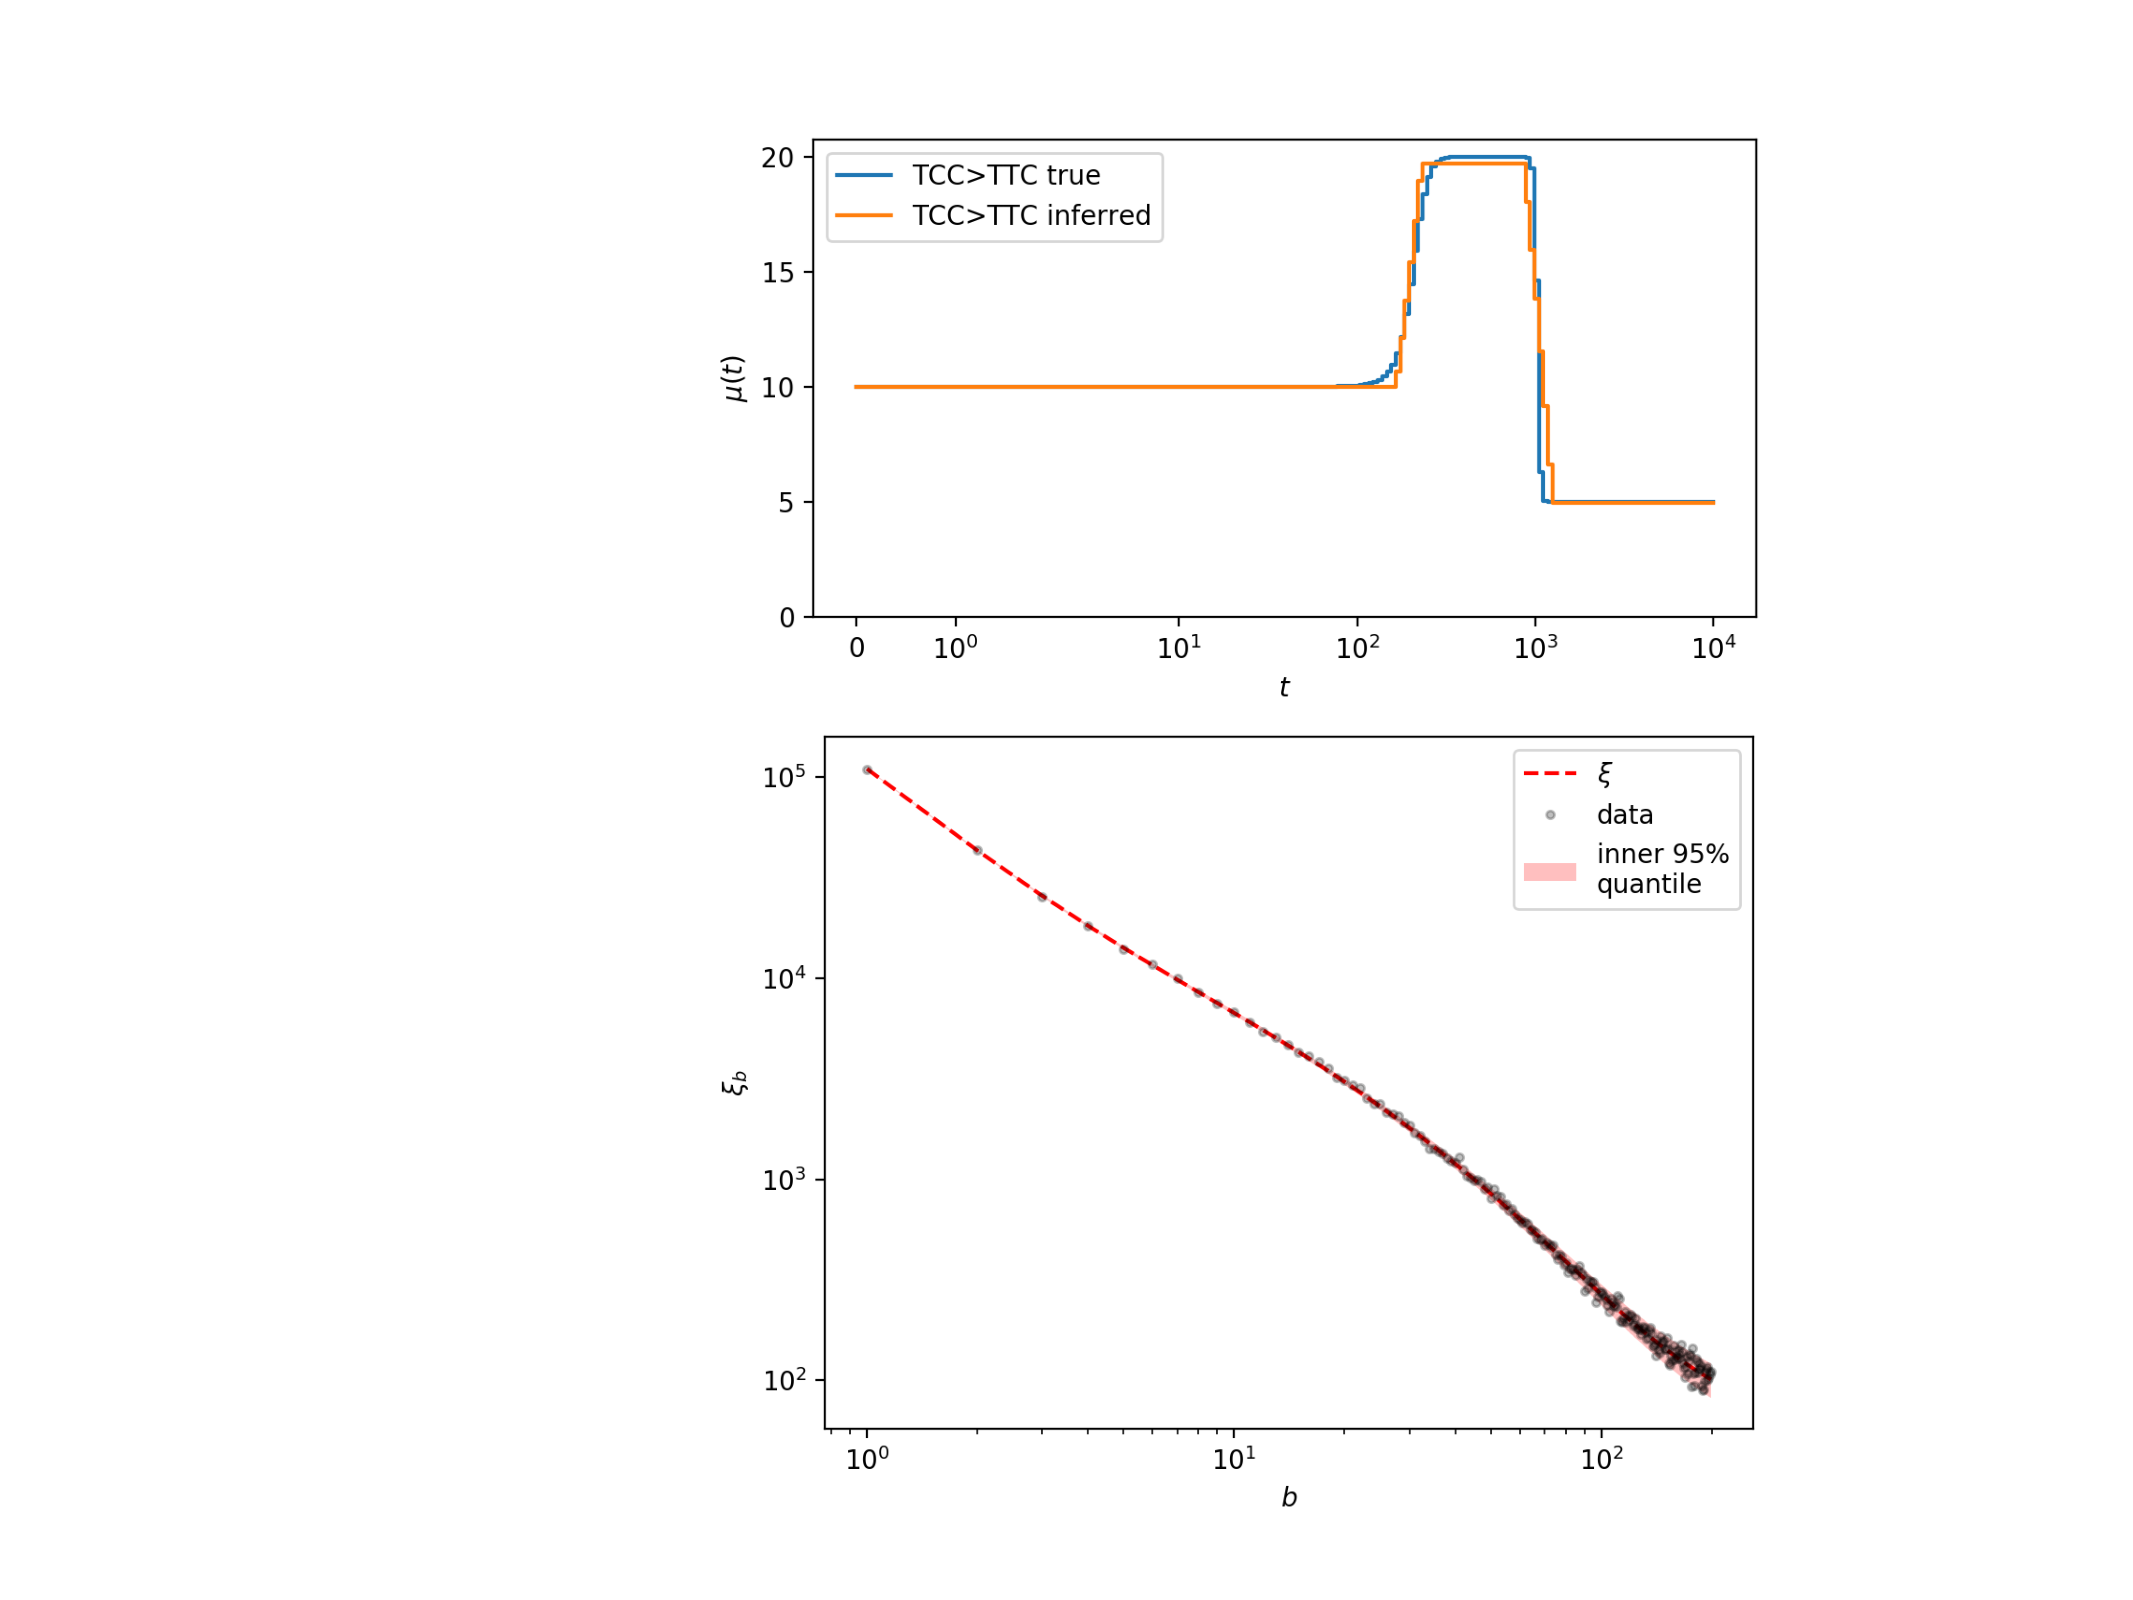
\includegraphics[width=.7\textwidth]{figures/fit_teaser}
  \caption{Simulating and inverting a pulse.}
  \label{}
\end{figure}

Todo:
\begin{itemize}
\item repeat 1KG analysis like in \cite{Harris2017-fw}, see if we recapitulate Kelley's simulation-based pulse results
\item cluster triplet time series to see if we pull in minor components.
\end{itemize}


\section{Discussion}\label{sec:discussion}

\section{Acknowledgements}\label{sec:ack}
Jean Feng suggested ADMM (if we end up using that).

\bibliographystyle{plainnat}
\bibliography{refs}






\end{document}
